\documentclass[../main.tex]{subfiles}
\graphicspath{{figures/}{../figures/}}

\begin{document}
% \todo[color=green!40]{完成问题三模型的求解(sections/q3\_solution)}

类似问题2使用模拟退火算法对问题3的单目标优化模型进行求解。具体步骤如下:

\noindent\textbf{步骤1 $\,\,$初始化参数和约束条件} 

设定导弹、干扰弹的初始位置与运动参数,构建三维空间中的动态几何关系。根据模型分析对发射参数设定合理边界。

\noindent\textbf{步骤2$\,\,$定义遮蔽判定函数和离散化时间轴}

通过模型分析中的几何条件判断干扰弹是否在某一时刻对导弹实现有效遮蔽,据此定义核心判别函数。将导弹飞行时间段划分为细小的时间步长,便于逐点判断遮蔽状态。

\noindent\textbf{步骤3 $\,\,$模拟退火搜索最优参数} 

根据发射角度、速度和时间参数,分阶段计算干扰弹的运动轨迹与云团的沉降轨迹,并更新其随时间变化的位置。
再利用判断函数判断各时刻是否有效,并统计出所有满足遮蔽条件的时间点,计算总持续时间作为目标函数。
采用与问题2类似的自适应模拟退火算法,通过随机扰动、接受准则和温度退火机制,全局搜索最优参数组合。
当优化停滞时,从历史搜索的优质解中重启搜索,增强跳出局部极值的能力。

\noindent\textbf{步骤4 $\,\,$输出最优遮蔽方案} 

返回最大遮蔽时间及对应的干扰弹投放参数,完成优化求解。

按照上述步骤,利用Python求解得到结果,见表\ref{tab:001}和表\ref{tab:031}.
\begin{table}[H]
\caption{问题3无人机投放策略}
\label{tab:001} 
\centering
\begin{small}
\begin{tabular}{ccccc}
\toprule[1.5pt]
无人机运动方向 & 无人机运动速度 & 烟幕干扰弹编号 & 烟幕干扰弹投放点的x坐标& 烟幕干扰弹投放点的y坐标 \\
\midrule[1pt]
  179.66           &140.00                  & 1     & 17653.00                   & 0.88     \\            
  179.66           &140.00                  & 2     & 17294.61                   & 3.03      \\           
  179.66          &140.00                  & 3     & 17112.61                   & 4.12      \\           
\bottomrule[1.5pt]
\end{tabular}
\end{small}
\end{table}

\begin{table}[H]
\caption{问题3无人机投放策略}
\label{tab:031} 
\centering
\begin{small}
\begin{tabular}{ccccc}
\toprule[1.5pt]
    干扰弹投放点的z坐标 &干扰弹起爆点的x坐标&干扰弹起爆点的y坐标&干扰弹起爆点的z坐标&有效干扰时长\\
\midrule[1pt]
1800.00             &17053.81                   & 4.47    &1710.23        & 4.1  \\               
1800.00             &16554.02                   & 7.47    & 1662.88       & 2.7  \\               
1800.00             &16290.83                   & 9.04    & 1631.16       & 1.7  \\                
\bottomrule[1.5pt]
\end{tabular}
\end{small}
\end{table}

\begin{figure}[H]
\centering
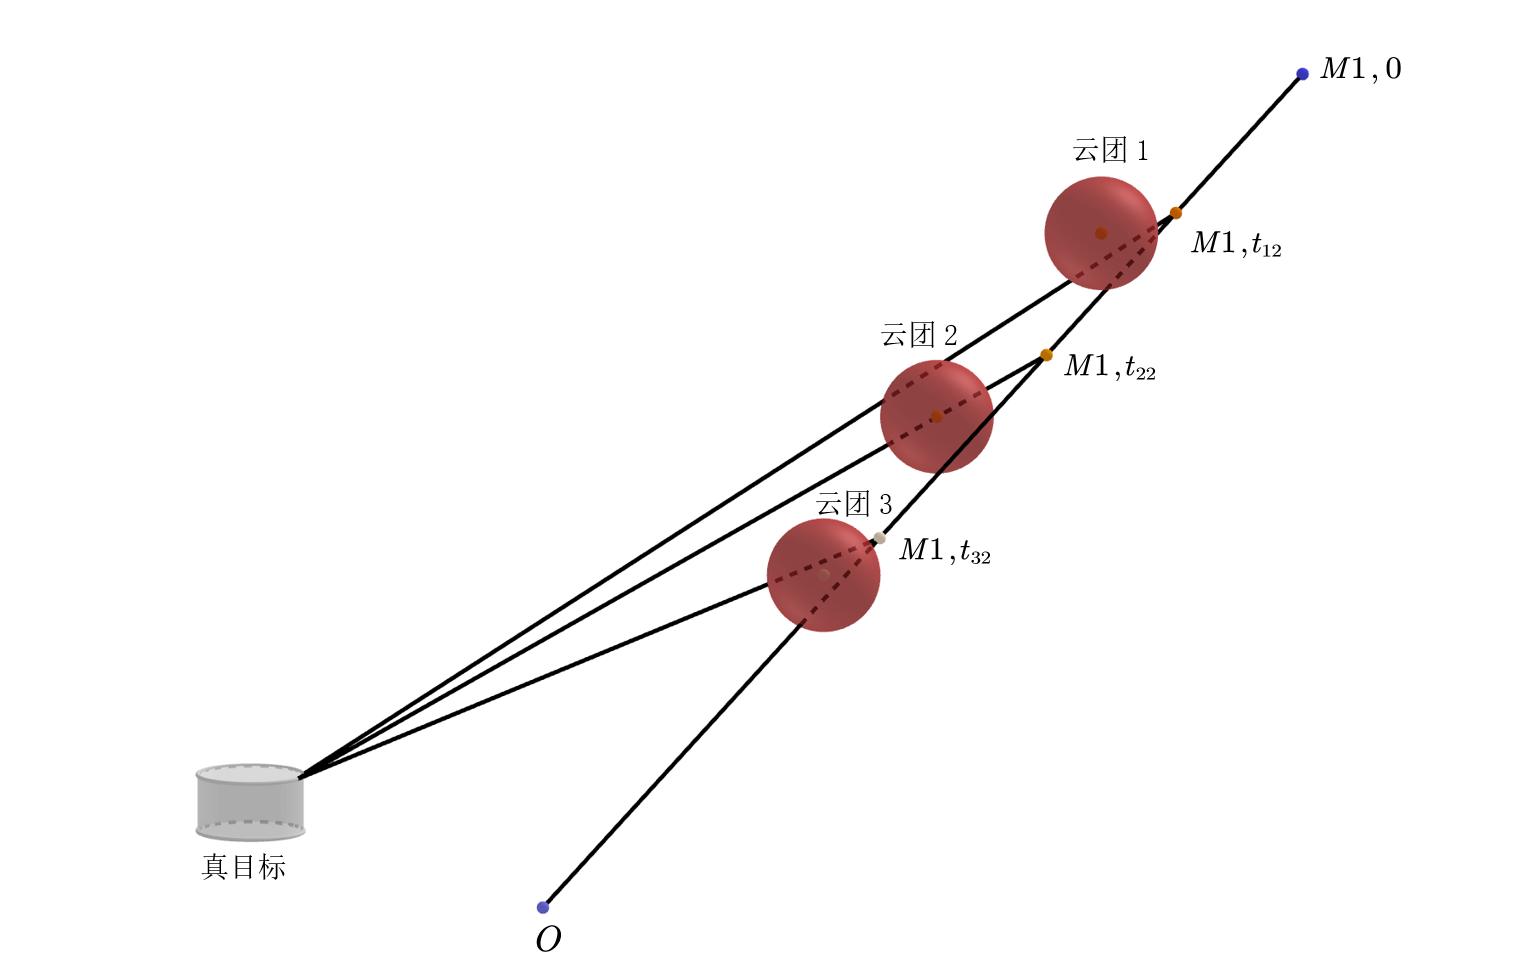
\includegraphics[scale=0.5]{图二.png}
\caption{}
\label{图2}
\end{figure}

\end{document}